\documentclass[11pt,compress,t,notes=noshow, xcolor=table]{beamer}
\documentclass[11pt,compress,t,notes=noshow, xcolor=table]{beamer}
\usepackage[]{graphicx}\usepackage[]{color}
% maxwidth is the original width if it is less than linewidth
% otherwise use linewidth (to make sure the graphics do not exceed the margin)
\makeatletter
\def\maxwidth{ %
  \ifdim\Gin@nat@width>\linewidth
    \linewidth
  \else
    \Gin@nat@width
  \fi
}
\makeatother

\definecolor{fgcolor}{rgb}{0.345, 0.345, 0.345}
\newcommand{\hlnum}[1]{\textcolor[rgb]{0.686,0.059,0.569}{#1}}%
\newcommand{\hlstr}[1]{\textcolor[rgb]{0.192,0.494,0.8}{#1}}%
\newcommand{\hlcom}[1]{\textcolor[rgb]{0.678,0.584,0.686}{\textit{#1}}}%
\newcommand{\hlopt}[1]{\textcolor[rgb]{0,0,0}{#1}}%
\newcommand{\hlstd}[1]{\textcolor[rgb]{0.345,0.345,0.345}{#1}}%
\newcommand{\hlkwa}[1]{\textcolor[rgb]{0.161,0.373,0.58}{\textbf{#1}}}%
\newcommand{\hlkwb}[1]{\textcolor[rgb]{0.69,0.353,0.396}{#1}}%
\newcommand{\hlkwc}[1]{\textcolor[rgb]{0.333,0.667,0.333}{#1}}%
\newcommand{\hlkwd}[1]{\textcolor[rgb]{0.737,0.353,0.396}{\textbf{#1}}}%
\let\hlipl\hlkwb

\usepackage{framed}
\makeatletter
\newenvironment{kframe}{%
 \def\at@end@of@kframe{}%
 \ifinner\ifhmode%
  \def\at@end@of@kframe{\end{minipage}}%
  \begin{minipage}{\columnwidth}%
 \fi\fi%
 \def\FrameCommand##1{\hskip\@totalleftmargin \hskip-\fboxsep
 \colorbox{shadecolor}{##1}\hskip-\fboxsep
     % There is no \\@totalrightmargin, so:
     \hskip-\linewidth \hskip-\@totalleftmargin \hskip\columnwidth}%
 \MakeFramed {\advance\hsize-\width
   \@totalleftmargin\z@ \linewidth\hsize
   \@setminipage}}%
 {\par\unskip\endMakeFramed%
 \at@end@of@kframe}
\makeatother

\definecolor{shadecolor}{rgb}{.97, .97, .97}
\definecolor{messagecolor}{rgb}{0, 0, 0}
\definecolor{warningcolor}{rgb}{1, 0, 1}
\definecolor{errorcolor}{rgb}{1, 0, 0}
\newenvironment{knitrout}{}{} % an empty environment to be redefined in TeX

\usepackage{alltt}
\newcommand{\SweaveOpts}[1]{}  % do not interfere with LaTeX
\newcommand{\SweaveInput}[1]{} % because they are not real TeX commands
\newcommand{\Sexpr}[1]{}       % will only be parsed by R
\newcommand{\xmark}{\ding{55}}%


\usepackage[english]{babel}
\usepackage[utf8]{inputenc}

\usepackage{dsfont}
\usepackage{verbatim}
\usepackage{amsmath}
\usepackage{amsfonts}
\usepackage{amssymb}
\usepackage{bm}
\usepackage{csquotes}
\usepackage{multirow}
\usepackage{longtable}
\usepackage{booktabs}
\usepackage{enumerate}
\usepackage[absolute,overlay]{textpos}
\usepackage{psfrag}
\usepackage{algorithm}
\usepackage{algpseudocode}
\usepackage{eqnarray}
\usepackage{arydshln}
\usepackage{tabularx}
\usepackage{placeins}
\usepackage{tikz}
\usepackage{setspace}
\usepackage{colortbl}
\usepackage{mathtools}
\usepackage{wrapfig}
\usepackage{bm}
\usepackage{amsmath}
\usepackage{pifont}

\usetikzlibrary{shapes,arrows,automata,positioning,calc,chains,trees, shadows}
\tikzset{
  %Define standard arrow tip
  >=stealth',
  %Define style for boxes
  punkt/.style={
    rectangle,
    rounded corners,
    draw=black, very thick,
    text width=6.5em,
    minimum height=2em,
    text centered},
  % Define arrow style
  pil/.style={
    ->,
    thick,
    shorten <=2pt,
    shorten >=2pt,}
}

\usepackage{subfig}

% Defines macros and environments
\usepackage{../../style/lmu-lecture}


\let\code=\texttt
\let\proglang=\textsf

\setkeys{Gin}{width=0.9\textwidth}

\setbeamertemplate{frametitle}{\expandafter\uppercase\expandafter\insertframetitle}

% This file is included in slides and exercises

% Rarely used fontstyle for R packages, used only in 
% - forests/slides-forests-benchmark.tex
% - exercises/single-exercises/methods_l_1.Rnw
% - slides/cart/attic/slides_extra_trees.Rnw
\newcommand{\pkg}[1]{{\fontseries{b}\selectfont #1}}

% Spacing helpers, used often (mostly in exercises for \dlz)
\newcommand{\lz}{\vspace{0.5cm}} % vertical space (used often in slides)
\newcommand{\dlz}{\vspace{1cm}}  % double vertical space (used often in exercises, never in slides)
\newcommand{\oneliner}[1] % Oneliner for important statements, used e.g. in iml, algods
{\begin{block}{}\begin{center}\begin{Large}#1\end{Large}\end{center}\end{block}}

% Don't know if this is used or needed, remove?
% textcolor that works in mathmode
% https://tex.stackexchange.com/a/261480
% Used e.g. in forests/slides-forests-bagging.tex
% [...] \textcolor{blue}{\tfrac{1}{M}\sum^M_{m} [...]
% \makeatletter
% \renewcommand*{\@textcolor}[3]{%
%   \protect\leavevmode
%   \begingroup
%     \color#1{#2}#3%
%   \endgroup
% }
% \makeatother






% latex-math includes as needed
% dependencies: amsmath, amssymb, dsfont
% math spaces
\ifdefined\N
\renewcommand{\N}{\mathds{N}} % N, naturals
\else \newcommand{\N}{\mathds{N}} \fi
\newcommand{\Z}{\mathds{Z}} % Z, integers
\newcommand{\Q}{\mathds{Q}} % Q, rationals
\newcommand{\R}{\mathds{R}} % R, reals
\ifdefined\C
\renewcommand{\C}{\mathds{C}} % C, complex
\else \newcommand{\C}{\mathds{C}} \fi
\newcommand{\continuous}{\mathcal{C}} % C, space of continuous functions
\newcommand{\M}{\mathcal{M}} % machine numbers
\newcommand{\epsm}{\epsilon_m} % maximum error

% counting / finite sets
\newcommand{\setzo}{\{0, 1\}} % set 0, 1
\newcommand{\setmp}{\{-1, +1\}} % set -1, 1
\newcommand{\unitint}{[0, 1]} % unit interval

% basic math stuff
\newcommand{\xt}{\tilde x} % x tilde
\newcommand{\argmin}{\mathop{\mathrm{arg\,min}}} % argmin
\newcommand{\argmax}{\mathop{\mathrm{arg\,max}}} % argmax
\newcommand{\argminlim}{\argmin\limits} % argmin with limits
\newcommand{\argmaxlim}{\argmax\limits} % argmax with limits
\newcommand{\sign}{\operatorname{sign}} % sign, signum
\newcommand{\I}{\mathbb{I}} % I, indicator
\newcommand{\order}{\mathcal{O}} % O, order
\newcommand{\bigO}{\mathcal{O}} % Big-O Landau
\newcommand{\littleo}{{o}} % Little-o Landau
\newcommand{\pd}[2]{\frac{\partial{#1}}{\partial #2}} % partial derivative
\newcommand{\floorlr}[1]{\left\lfloor #1 \right\rfloor} % floor
\newcommand{\ceillr}[1]{\left\lceil #1 \right\rceil} % ceiling
\newcommand{\indep}{\perp \!\!\! \perp} % independence symbol

% sums and products
\newcommand{\sumin}{\sum\limits_{i=1}^n} % summation from i=1 to n
\newcommand{\sumim}{\sum\limits_{i=1}^m} % summation from i=1 to m
\newcommand{\sumjn}{\sum\limits_{j=1}^n} % summation from j=1 to p
\newcommand{\sumjp}{\sum\limits_{j=1}^p} % summation from j=1 to p
\newcommand{\sumik}{\sum\limits_{i=1}^k} % summation from i=1 to k
\newcommand{\sumkg}{\sum\limits_{k=1}^g} % summation from k=1 to g
\newcommand{\sumjg}{\sum\limits_{j=1}^g} % summation from j=1 to g
\newcommand{\summM}{\sum\limits_{m=1}^M} % summation from m=1 to M
\newcommand{\meanin}{\frac{1}{n} \sum\limits_{i=1}^n} % mean from i=1 to n
\newcommand{\meanim}{\frac{1}{m} \sum\limits_{i=1}^m} % mean from i=1 to n
\newcommand{\meankg}{\frac{1}{g} \sum\limits_{k=1}^g} % mean from k=1 to g
\newcommand{\meanmM}{\frac{1}{M} \sum\limits_{m=1}^M} % mean from m=1 to M
\newcommand{\prodin}{\prod\limits_{i=1}^n} % product from i=1 to n
\newcommand{\prodkg}{\prod\limits_{k=1}^g} % product from k=1 to g
\newcommand{\prodjp}{\prod\limits_{j=1}^p} % product from j=1 to p

% linear algebra
\newcommand{\one}{\bm{1}} % 1, unitvector
\newcommand{\zero}{\mathbf{0}} % 0-vector
\newcommand{\id}{\bm{I}} % I, identity
\newcommand{\diag}{\operatorname{diag}} % diag, diagonal
\newcommand{\trace}{\operatorname{tr}} % tr, trace
\newcommand{\spn}{\operatorname{span}} % span
\newcommand{\scp}[2]{\left\langle #1, #2 \right\rangle} % <.,.>, scalarproduct
\newcommand{\mat}[1]{\begin{pmatrix} #1 \end{pmatrix}} % short pmatrix command
\newcommand{\Amat}{\mathbf{A}} % matrix A
\newcommand{\Deltab}{\mathbf{\Delta}} % error term for vectors

% basic probability + stats
\renewcommand{\P}{\mathds{P}} % P, probability
\newcommand{\E}{\mathds{E}} % E, expectation
\newcommand{\var}{\mathsf{Var}} % Var, variance
\newcommand{\cov}{\mathsf{Cov}} % Cov, covariance
\newcommand{\corr}{\mathsf{Corr}} % Corr, correlation
\newcommand{\normal}{\mathcal{N}} % N of the normal distribution
\newcommand{\iid}{\overset{i.i.d}{\sim}} % dist with i.i.d superscript
\newcommand{\distas}[1]{\overset{#1}{\sim}} % ... is distributed as ...

% machine learning
\newcommand{\Xspace}{\mathcal{X}} % X, input space
\newcommand{\Yspace}{\mathcal{Y}} % Y, output space
\newcommand{\Zspace}{\mathcal{Z}} % Z, space of sampled datapoints
\newcommand{\nset}{\{1, \ldots, n\}} % set from 1 to n
\newcommand{\pset}{\{1, \ldots, p\}} % set from 1 to p
\newcommand{\gset}{\{1, \ldots, g\}} % set from 1 to g
\newcommand{\Pxy}{\mathbb{P}_{xy}} % P_xy
\newcommand{\Exy}{\mathbb{E}_{xy}} % E_xy: Expectation over random variables xy
\newcommand{\xv}{\mathbf{x}} % vector x (bold)
\newcommand{\xtil}{\tilde{\mathbf{x}}} % vector x-tilde (bold)
\newcommand{\yv}{\mathbf{y}} % vector y (bold)
\newcommand{\xy}{(\xv, y)} % observation (x, y)
\newcommand{\xvec}{\left(x_1, \ldots, x_p\right)^\top} % (x1, ..., xp)
\newcommand{\Xmat}{\mathbf{X}} % Design matrix
\newcommand{\allDatasets}{\mathds{D}} % The set of all datasets
\newcommand{\allDatasetsn}{\mathds{D}_n}  % The set of all datasets of size n
\newcommand{\D}{\mathcal{D}} % D, data
\newcommand{\Dn}{\D_n} % D_n, data of size n
\newcommand{\Dtrain}{\mathcal{D}_{\text{train}}} % D_train, training set
\newcommand{\Dtest}{\mathcal{D}_{\text{test}}} % D_test, test set
\newcommand{\xyi}[1][i]{\left(\xv^{(#1)}, y^{(#1)}\right)} % (x^i, y^i), i-th observation
\newcommand{\Dset}{\left( \xyi[1], \ldots, \xyi[n]\right)} % {(x1,y1)), ..., (xn,yn)}, data
\newcommand{\defAllDatasetsn}{(\Xspace \times \Yspace)^n} % Def. of the set of all datasets of size n
\newcommand{\defAllDatasets}{\bigcup_{n \in \N}(\Xspace \times \Yspace)^n} % Def. of the set of all datasets
\newcommand{\xdat}{\left\{ \xv^{(1)}, \ldots, \xv^{(n)}\right\}} % {x1, ..., xn}, input data
\newcommand{\ydat}{\left\{ \yv^{(1)}, \ldots, \yv^{(n)}\right\}} % {y1, ..., yn}, input data
\newcommand{\yvec}{\left(y^{(1)}, \hdots, y^{(n)}\right)^\top} % (y1, ..., yn), vector of outcomes
\newcommand{\greekxi}{\xi} % Greek letter xi
\renewcommand{\xi}[1][i]{\xv^{(#1)}} % x^i, i-th observed value of x
\newcommand{\yi}[1][i]{y^{(#1)}} % y^i, i-th observed value of y
\newcommand{\xivec}{\left(x^{(i)}_1, \ldots, x^{(i)}_p\right)^\top} % (x1^i, ..., xp^i), i-th observation vector
\newcommand{\xj}{\xv_j} % x_j, j-th feature
\newcommand{\xjvec}{\left(x^{(1)}_j, \ldots, x^{(n)}_j\right)^\top} % (x^1_j, ..., x^n_j), j-th feature vector
\newcommand{\phiv}{\mathbf{\phi}} % Basis transformation function phi
\newcommand{\phixi}{\mathbf{\phi}^{(i)}} % Basis transformation of xi: phi^i := phi(xi)

%%%%%% ml - models general
\newcommand{\lamv}{\bm{\lambda}} % lambda vector, hyperconfiguration vector
\newcommand{\Lam}{\bm{\Lambda}}	 % Lambda, space of all hpos
% Inducer / Inducing algorithm
\newcommand{\preimageInducer}{\left(\defAllDatasets\right)\times\Lam} % Set of all datasets times the hyperparameter space
\newcommand{\preimageInducerShort}{\allDatasets\times\Lam} % Set of all datasets times the hyperparameter space
% Inducer / Inducing algorithm
\newcommand{\ind}{\mathcal{I}} % Inducer, inducing algorithm, learning algorithm

% continuous prediction function f
\newcommand{\ftrue}{f_{\text{true}}}  % True underlying function (if a statistical model is assumed)
\newcommand{\ftruex}{\ftrue(\xv)} % True underlying function (if a statistical model is assumed)
\newcommand{\fx}{f(\xv)} % f(x), continuous prediction function
\newcommand{\fdomains}{f: \Xspace \rightarrow \R^g} % f with domain and co-domain
\newcommand{\Hspace}{\mathcal{H}} % hypothesis space where f is from
\newcommand{\fbayes}{f^{\ast}} % Bayes-optimal model
\newcommand{\fxbayes}{f^{\ast}(\xv)} % Bayes-optimal model
\newcommand{\fkx}[1][k]{f_{#1}(\xv)} % f_j(x), discriminant component function
\newcommand{\fh}{\hat{f}} % f hat, estimated prediction function
\newcommand{\fxh}{\fh(\xv)} % fhat(x)
\newcommand{\fxt}{f(\xv ~|~ \thetav)} % f(x | theta)
\newcommand{\fxi}{f\left(\xv^{(i)}\right)} % f(x^(i))
\newcommand{\fxih}{\hat{f}\left(\xv^{(i)}\right)} % f(x^(i))
\newcommand{\fxit}{f\left(\xv^{(i)} ~|~ \thetav\right)} % f(x^(i) | theta)
\newcommand{\fhD}{\fh_{\D}} % fhat_D, estimate of f based on D
\newcommand{\fhDtrain}{\fh_{\Dtrain}} % fhat_Dtrain, estimate of f based on D
\newcommand{\fhDnlam}{\fh_{\Dn, \lamv}} %model learned on Dn with hp lambda
\newcommand{\fhDlam}{\fh_{\D, \lamv}} %model learned on D with hp lambda
\newcommand{\fhDnlams}{\fh_{\Dn, \lamv^\ast}} %model learned on Dn with optimal hp lambda
\newcommand{\fhDlams}{\fh_{\D, \lamv^\ast}} %model learned on D with optimal hp lambda

% discrete prediction function h
\newcommand{\hx}{h(\xv)} % h(x), discrete prediction function
\newcommand{\hh}{\hat{h}} % h hat
\newcommand{\hxh}{\hat{h}(\xv)} % hhat(x)
\newcommand{\hxt}{h(\xv | \thetav)} % h(x | theta)
\newcommand{\hxi}{h\left(\xi\right)} % h(x^(i))
\newcommand{\hxit}{h\left(\xi ~|~ \thetav\right)} % h(x^(i) | theta)
\newcommand{\hbayes}{h^{\ast}} % Bayes-optimal classification model
\newcommand{\hxbayes}{h^{\ast}(\xv)} % Bayes-optimal classification model

% yhat
\newcommand{\yh}{\hat{y}} % yhat for prediction of target
\newcommand{\yih}{\hat{y}^{(i)}} % yhat^(i) for prediction of ith targiet
\newcommand{\resi}{\yi- \yih}

% theta
\newcommand{\thetah}{\hat{\theta}} % theta hat
\newcommand{\thetav}{\bm{\theta}} % theta vector
\newcommand{\thetavh}{\bm{\hat\theta}} % theta vector hat
\newcommand{\thetat}[1][t]{\thetav^{[#1]}} % theta^[t] in optimization
\newcommand{\thetatn}[1][t]{\thetav^{[#1 +1]}} % theta^[t+1] in optimization
\newcommand{\thetahDnlam}{\thetavh_{\Dn, \lamv}} %theta learned on Dn with hp lambda
\newcommand{\thetahDlam}{\thetavh_{\D, \lamv}} %theta learned on D with hp lambda
\newcommand{\mint}{\min_{\thetav \in \Theta}} % min problem theta
\newcommand{\argmint}{\argmin_{\thetav \in \Theta}} % argmin theta

% densities + probabilities
% pdf of x
\newcommand{\pdf}{p} % p
\newcommand{\pdfx}{p(\xv)} % p(x)
\newcommand{\pixt}{\pi(\xv~|~ \thetav)} % pi(x|theta), pdf of x given theta
\newcommand{\pixit}[1][i]{\pi\left(\xi[#1] ~|~ \thetav\right)} % pi(x^i|theta), pdf of x given theta
\newcommand{\pixii}[1][i]{\pi\left(\xi[#1]\right)} % pi(x^i), pdf of i-th x

% pdf of (x, y)
\newcommand{\pdfxy}{p(\xv,y)} % p(x, y)
\newcommand{\pdfxyt}{p(\xv, y ~|~ \thetav)} % p(x, y | theta)
\newcommand{\pdfxyit}{p\left(\xi, \yi ~|~ \thetav\right)} % p(x^(i), y^(i) | theta)

% pdf of x given y
\newcommand{\pdfxyk}[1][k]{p(\xv | y= #1)} % p(x | y = k)
\newcommand{\lpdfxyk}[1][k]{\log p(\xv | y= #1)} % log p(x | y = k)
\newcommand{\pdfxiyk}[1][k]{p\left(\xi | y= #1 \right)} % p(x^i | y = k)

% prior probabilities
\newcommand{\pik}[1][k]{\pi_{#1}} % pi_k, prior
\newcommand{\lpik}[1][k]{\log \pi_{#1}} % log pi_k, log of the prior
\newcommand{\pit}{\pi(\thetav)} % Prior probability of parameter theta

% posterior probabilities
\newcommand{\post}{\P(y = 1 ~|~ \xv)} % P(y = 1 | x), post. prob for y=1
\newcommand{\postk}[1][k]{\P(y = #1 ~|~ \xv)} % P(y = k | y), post. prob for y=k
\newcommand{\pidomains}{\pi: \Xspace \rightarrow \unitint} % pi with domain and co-domain
\newcommand{\pibayes}{\pi^{\ast}} % Bayes-optimal classification model
\newcommand{\pixbayes}{\pi^{\ast}(\xv)} % Bayes-optimal classification model
\newcommand{\pix}{\pi(\xv)} % pi(x), P(y = 1 | x)
\newcommand{\piv}{\bm{\pi}} % pi, bold, as vector
\newcommand{\pikx}[1][k]{\pi_{#1}(\xv)} % pi_k(x), P(y = k | x)
\newcommand{\pikxt}[1][k]{\pi_{#1}(\xv ~|~ \thetav)} % pi_k(x | theta), P(y = k | x, theta)
\newcommand{\pixh}{\hat \pi(\xv)} % pi(x) hat, P(y = 1 | x) hat
\newcommand{\pikxh}[1][k]{\hat \pi_{#1}(\xv)} % pi_k(x) hat, P(y = k | x) hat
\newcommand{\pixih}{\hat \pi(\xi)} % pi(x^(i)) with hat
\newcommand{\pikxih}[1][k]{\hat \pi_{#1}(\xi)} % pi_k(x^(i)) with hat
\newcommand{\pdfygxt}{p(y ~|~\xv, \thetav)} % p(y | x, theta)
\newcommand{\pdfyigxit}{p\left(\yi ~|~\xi, \thetav\right)} % p(y^i |x^i, theta)
\newcommand{\lpdfygxt}{\log \pdfygxt } % log p(y | x, theta)
\newcommand{\lpdfyigxit}{\log \pdfyigxit} % log p(y^i |x^i, theta)

% probababilistic
\newcommand{\bayesrulek}[1][k]{\frac{\P(\xv | y= #1) \P(y= #1)}{\P(\xv)}} % Bayes rule
\newcommand{\muk}{\bm{\mu_k}} % mean vector of class-k Gaussian (discr analysis)

% residual and margin
\newcommand{\eps}{\epsilon} % residual, stochastic
\newcommand{\epsv}{\bm{\epsilon}} % residual, stochastic, as vector
\newcommand{\epsi}{\epsilon^{(i)}} % epsilon^i, residual, stochastic
\newcommand{\epsh}{\hat{\epsilon}} % residual, estimated
\newcommand{\epsvh}{\hat{\epsv}} % residual, estimated, vector
\newcommand{\yf}{y \fx} % y f(x), margin
\newcommand{\yfi}{\yi \fxi} % y^i f(x^i), margin
\newcommand{\Sigmah}{\hat \Sigma} % estimated covariance matrix
\newcommand{\Sigmahj}{\hat \Sigma_j} % estimated covariance matrix for the j-th class

% ml - loss, risk, likelihood
\newcommand{\Lyf}{L\left(y, f\right)} % L(y, f), loss function
\newcommand{\Lypi}{L\left(y, \pi\right)} % L(y, pi), loss function
\newcommand{\Lxy}{L\left(y, \fx\right)} % L(y, f(x)), loss function
\newcommand{\Lxyi}{L\left(\yi, \fxi\right)} % loss of observation
\newcommand{\Lxyt}{L\left(y, \fxt\right)} % loss with f parameterized
\newcommand{\Lxyit}{L\left(\yi, \fxit\right)} % loss of observation with f parameterized
\newcommand{\Lxym}{L\left(\yi, f\left(\bm{\tilde{x}}^{(i)} ~|~ \thetav\right)\right)} % loss of observation with f parameterized
\newcommand{\Lpixy}{L\left(y, \pix\right)} % loss in classification
\newcommand{\Lpiy}{L\left(y, \pi\right)} % loss in classification
\newcommand{\Lpiv}{L\left(y, \piv\right)} % loss in classification
\newcommand{\Lpixyi}{L\left(\yi, \pixii\right)} % loss of observation in classification
\newcommand{\Lpixyt}{L\left(y, \pixt\right)} % loss with pi parameterized
\newcommand{\Lpixyit}{L\left(\yi, \pixit\right)} % loss of observation with pi parameterized
\newcommand{\Lhy}{L\left(y, h\right)} % L(y, h), loss function on discrete classes
\newcommand{\Lhxy}{L\left(y, \hx\right)} % L(y, h(x)), loss function on discrete classes
\newcommand{\Lr}{L\left(r\right)} % L(r), loss defined on residual (reg) / margin (classif)
\newcommand{\lone}{|y - \fx|} % L1 loss
\newcommand{\ltwo}{\left(y - \fx\right)^2} % L2 loss
\newcommand{\lbernoullimp}{\ln(1 + \exp(-y \cdot \fx))} % Bernoulli loss for -1, +1 encoding
\newcommand{\lbernoullizo}{- y \cdot \fx + \log(1 + \exp(\fx))} % Bernoulli loss for 0, 1 encoding
\newcommand{\lcrossent}{- y \log \left(\pix\right) - (1 - y) \log \left(1 - \pix\right)} % cross-entropy loss
\newcommand{\lbrier}{\left(\pix - y \right)^2} % Brier score
\newcommand{\risk}{\mathcal{R}} % R, risk
\newcommand{\riskbayes}{\mathcal{R}^\ast}
\newcommand{\riskf}{\risk(f)} % R(f), risk
\newcommand{\riskdef}{\E_{y|\xv}\left(\Lxy \right)} % risk def (expected loss)
\newcommand{\riskt}{\mathcal{R}(\thetav)} % R(theta), risk
\newcommand{\riske}{\mathcal{R}_{\text{emp}}} % R_emp, empirical risk w/o factor 1 / n
\newcommand{\riskeb}{\bar{\mathcal{R}}_{\text{emp}}} % R_emp, empirical risk w/ factor 1 / n
\newcommand{\riskef}{\riske(f)} % R_emp(f)
\newcommand{\risket}{\mathcal{R}_{\text{emp}}(\thetav)} % R_emp(theta)
\newcommand{\riskr}{\mathcal{R}_{\text{reg}}} % R_reg, regularized risk
\newcommand{\riskrt}{\mathcal{R}_{\text{reg}}(\thetav)} % R_reg(theta)
\newcommand{\riskrf}{\riskr(f)} % R_reg(f)
\newcommand{\riskrth}{\hat{\mathcal{R}}_{\text{reg}}(\thetav)} % hat R_reg(theta)
\newcommand{\risketh}{\hat{\mathcal{R}}_{\text{emp}}(\thetav)} % hat R_emp(theta)
\newcommand{\LL}{\mathcal{L}} % L, likelihood
\newcommand{\LLt}{\mathcal{L}(\thetav)} % L(theta), likelihood
\newcommand{\LLtx}{\mathcal{L}(\thetav | \xv)} % L(theta|x), likelihood
\newcommand{\logl}{\ell} % l, log-likelihood
\newcommand{\loglt}{\logl(\thetav)} % l(theta), log-likelihood
\newcommand{\logltx}{\logl(\thetav | \xv)} % l(theta|x), log-likelihood
\newcommand{\errtrain}{\text{err}_{\text{train}}} % training error
\newcommand{\errtest}{\text{err}_{\text{test}}} % test error
\newcommand{\errexp}{\overline{\text{err}_{\text{test}}}} % avg training error

% lm
\newcommand{\thx}{\thetav^\top \xv} % linear model
\newcommand{\olsest}{(\Xmat^\top \Xmat)^{-1} \Xmat^\top \yv} % OLS estimator in LM


% Lecture title always has to be there
\title{Algorithms and Data Structures}

\begin{document}

\titlemeta{% Chunk title (example: CART, Forests, Boosting, ...), can be empty
Matrix Decomposition
}{% Lecture title
Overdetermined Systems \& Regression Example
}{% Relative path to title page image: Can be empty but must not start with slides/
}{% Learning goals, wrapped inside itemize environment
  \item Overdetermined systems
  \item Normal equation
  \item Regression
}
%\lecture{CIM1 Statistical Computing}

\begin{vbframe}{Overdetermined Systems}

A system of linear equations $\bm{Ax} = \bm{b}$ with $\bm{A} \in \R^{m\times n}, m \ge n$ with more equations than unknowns, is called \textbf{overdetermined}.

\lz

In general such a system has no (exact) solution.

\lz

A (compromise) solution using \textbf{least squares} is the vector $\bm{x}$ which minimizes the squared sum of the \textbf{residual vector} $\bm{r} = \mathbf{b} - \mathbf{A}\boldsymbol{x}$:

$$
\bm{x} = \text{arg} \min \|\mathbf{b} - \mathbf{A}\boldsymbol{x}\|^2_2
$$

\end{vbframe}

\begin{vbframe}{Example: the regression model}

\textbf{Aim:} Solve $\bm{X}\boldsymbol{\beta} = \bm{y}$ with

\begin{itemize}
\item $\mathbf{X}$: $n \times (p + 1)$, Design matrix
\item $\mathbf{y}$: $n \times 1$, $n$ observations
% \item $\boldsymbol{\varepsilon}$: $n \times 1$ Fehlerterm
\item $\boldsymbol{\beta}$: $(p + 1) \times 1$, $p$ regressors plus intercept
\end{itemize}

Since the linear system is usually overdetermined (more observations than variables) and has no solution, we minimize the residual sum of squares:

$$
\min_\beta \|\mathbf{y} - \mathbf{X}\boldsymbol{\beta}\|^2_2 = (\mathbf{y} - \mathbf{X}\boldsymbol{\beta})^\top
  (\mathbf{y} - \mathbf{X}\boldsymbol{\beta})
$$

\lz

\textbf{Questions}: How can the problem be solved in a numerically stable way? Which algorithms are fast?


% Matrizenschreibweise:
% $$
% \mathbf{y} = \mathbf{X}\boldsymbol{\beta} + \boldsymbol{\varepsilon},
%  \qquad \E(\boldsymbol{\varepsilon}) = \mathbf{0},
% $$
% \begin{itemize}
% \item $\mathbf{y}$: $n \times 1$ Zufallsvektor, $n$ Beobachtungen
% \item $\boldsymbol{\varepsilon}$: $n \times 1$ Fehlerterm
% \item $\boldsymbol{\beta}$: $(p + 1) \times 1$, $p$ Regressoren plus Intercept,
% \item $\mathbf{X}$: $n \times (p + 1)$, Design-Matrix (für uns fest).
% \end{itemize}
% Minimale Anforderungen an den Fehlerterm:
% \begin{itemize}
% \item Klassisches Modell: $\cov(\boldsymbol{\varepsilon}) = \sigma^2 \mathbf{I}$.
% \item Allgemeines lineares Modell: $\cov(\boldsymbol{\varepsilon}) = \boldsymbol{\Sigma}$.
% \end{itemize}
% \end{vbframe}

% \begin{vbframe}{Least Squares Regression}
% \textbf{Ziel:} Minimieren der Quadratsumme der Fehler
% $$
% \min_\beta \|\mathbf{y} - \mathbf{X}\boldsymbol{\beta}\|^2_2 = (\mathbf{y} - \mathbf{X}\boldsymbol{\beta})^\top
%   (\mathbf{y} - \mathbf{X}\boldsymbol{\beta}).
% $$



% Falls $\mathbf{X}$ vollen Rang hat $\quad \Rightarrow \quad \hat{\boldsymbol{\beta}} =
%   (\mathbf{X}^\top\mathbf{X})^{-1}\mathbf{X}^\top\mathbf{y}$.\\

% \framebreak
%
% Residuenvektor
% $$
% \mathbf{e} = \mathbf{y} - \hat{\mathbf{y}} = \mathbf{y} - \mathbf{X}\hat{\boldsymbol{\beta}} =
%   \mathbf{y} - \mathbf{X}(\mathbf{X}^\top\mathbf{X})^{-1}\mathbf{X}^\top\mathbf{y} =
%   (\mathbf{I} - \mathbf{P})\mathbf{y},
% $$
% wobei  $\mathbf{P} = \mathbf{X}(\mathbf{X}^\top\mathbf{X})^{-1}\mathbf{X}^\top$ symmetrisch und
% idempotent. \\
% $\quad \Rightarrow \quad$ \textbf{Projektionsoperator}\\
% \medskip
% $\mathbf{P}$ \dots Projektion auf linearen Unterraum, der von $\mathbf{X}$ aufgespannt \\
% $\mathbf{I} - \mathbf{P}$ \dots Projektion auf Orthogonalraum\\
% \medskip
% Damit gilt für Residual Sum of Squares:
% $$
% RSS = Q(\hat{\boldsymbol{\beta}}) = \mathbf{y}^\top(\mathbf{I} - \mathbf{P})^\top(\mathbf{I} -
%   \mathbf{P})\mathbf{y} =  \mathbf{y}^\top(\mathbf{I} - \mathbf{P})\mathbf{y}
% $$

% \framebreak

% Anschaulich kann man sich klar machen, dass die Differenz $\|\mathbf{r}(\boldsymbol{\beta})\| = \|\mathbf{y} - \mathbf{X}\boldsymbol{\beta}\|_2$ dann minimal wird, wenn $\mathbf{y} - \mathbf{X}\boldsymbol{\beta}$ senkrecht auf dem Bildraum von $\text{Bild}(\mathbf{X}) = \{\mathbf{X} \boldsymbol{\beta} | \boldsymbol{\beta} \in \R^{p+1}\}$ steht.

% \begin{center}
% 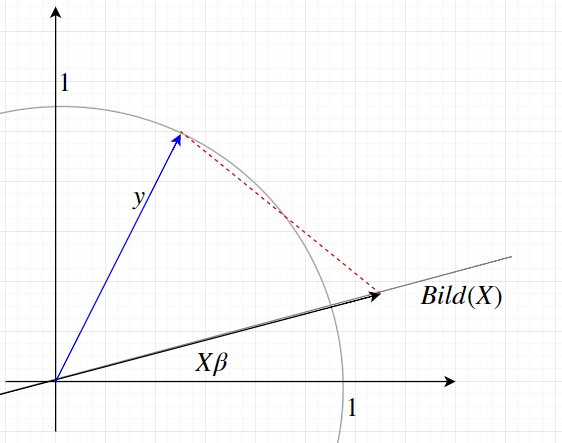
\includegraphics[width = 0.5\textwidth]{figure_man/ignore/regression.png} ~~ 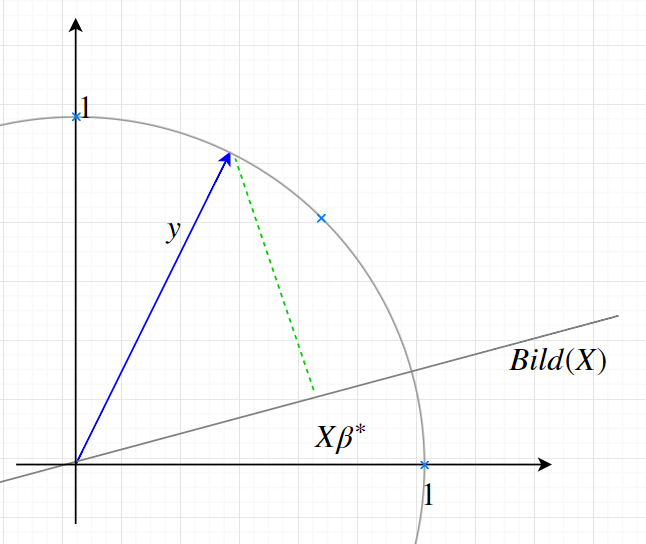
\includegraphics[width = 0.5\textwidth]{figure_man/ignore/regressionopt.png}
% \end{center}

% \end{vbframe}

% \begin{vbframe}{Kondition der Regression}

% Wir interessieren uns für die Berechnung des Parametervektors $\boldsymbol{\beta}$. Somit is $\boldsymbol{\beta}$ als Ergebnis und $\mathbf{y}$ bzw. $\mathbf{X}$ als Eingabe zu sehen.

% \lz

% Wie verändert sich das optimale $\boldsymbol{\beta}^*$ bei einer kleinen Störung von $\mathbf{y}$?


% \begin{center}
% 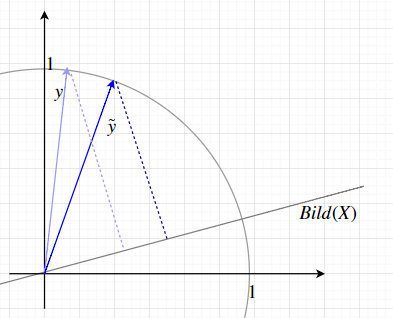
\includegraphics[width = 0.4\textwidth]{figure_man/ignore/regressionkonditionbad.png} ~~~ 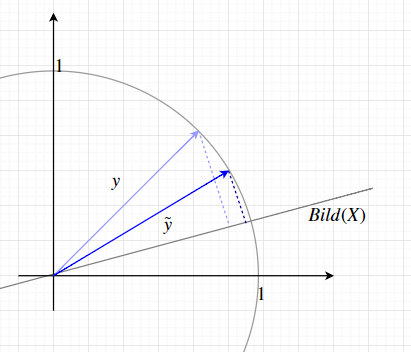
\includegraphics[width = 0.4\textwidth]{figure_man/ignore/regressionkonditiongood.png}
% \end{center}


% Notation:  $\tilde{\mathbf{y}} = \mathbf{y} + \Deltab \mathbf{y}$ eine kleine Abweichung von $\mathbf{y}$, $\boldsymbol{\beta}^*$ und $\tilde{\boldsymbol{\beta}}^*$ die jeweiligen Schätzer. \\

% \lz

% Dann gilt

% $$
% \frac{\|\boldsymbol{\beta}^* - \tilde{\boldsymbol{\beta}}^*\| }{\|\boldsymbol{\beta}^*\|}
%   \leq \frac{\kappa(\mathbf{X})}{\cos(\theta)} \frac{\|\Deltab \mathbf{y}\| }{\|{\mathbf{y}}\|}.
% $$

% Hierbei bezeichne

% \begin{itemize}
% \item $\kappa(\mathbf{X}):= \sqrt{\kappa(\mathbf{X}^T\mathbf{X})}$ die Kondition der $n \times (p + 1)$ Matrix $\mathbf{X}$,
% \item $\theta$ den Winkel zwischen $\mathbf{y}$ und dem Unterraum $\{\mathbf{X} \boldsymbol{\beta} | \boldsymbol{\beta} \in \R^{p+1}\}$.
% \end{itemize}

% Die Kondition des linearen Ausgleichsproblems bzgl. Störungen in $\mathbf{y}$ kann also abgeschätzt werden durch $\frac{\kappa(\mathbf{X})}{\cos(\theta)}$.

% \framebreak

% Bezüglich Störungen der Matrix $\tilde{\mathbf{X}} = \mathbf{X} + \Deltab \mathbf{X}$ ergibt sich ein etwas komplizierteres Resultat

% $$
% \frac{\|\boldsymbol{\beta}^* - \tilde{\boldsymbol{\beta}}^*\| }{\|\boldsymbol{\beta}^*\|}
%   \leq \biggl(\kappa(\mathbf{X}) + \kappa(\mathbf{X})^2\tan \theta\biggr) \frac{\|\Deltab \mathbf{X}\| }{\|{\mathbf{X}}\|}.
% $$

% Die Konditionszahl bzgl. Störungen in $\mathbf{X}$ lautet also

% $$
% \kappa(\mathbf{X}) + \kappa(\mathbf{X})^2\tan \theta.
% $$

% \vfill

% \begin{footnotesize}
% Eine Herleitung für obige Resultate ist hier zu finden:
% \emph{Deuflhard, Numerische Mathematik I, 2001, Kapitel 3}
% \end{footnotesize}

% \framebreak

% \begin{itemize}
% \item In beiden Formeln sieht man: Die Kondition des linearen Ausgleichsproblems hängt also nicht nur von der Kondition der Matrix $\mathbf{X}$, sondern auch von der Größe des Winkels $\theta$ und damit der Größe des Residuums $\mathbf{r} := \mathbf{y} - \mathbf{X} \boldsymbol{\beta}^*$ ab.
% \item Für kleine Residuen, also $\cos\theta \approx 1$ und $\tan \theta \approx 0$, verhält sich das lineare Ausgleichsproblem konditionell wie ein lineares Gleichungssystem.
% \item Für große Residuen, also $\cos \theta \ll 1$ und $\tan\theta \gg 1$, verhält sich das lineare Ausgleichsproblem konditionell wesentlich anders als lineare Gleichungssysteme.
% \end{itemize}

% wobei $\kappa^* := \sqrt{\kappa(\mathbf{X}^\top\mathbf{X})}$\\
% \medskip
% Nur Störungen von $\mathbf{y}$, die tatsächlich Einfluss auf die geschätzte Lösung haben,
% wirken sich auf geschätzte Koeffizienten aus $\quad \Rightarrow \quad$ sinnvolles Resultat für Regressionsdiagnostik.

\end{vbframe}

\begin{vbframe}{Condition of normal equations}

The solution of the optimization problem is (mathematically) equivalent to the solution of the \textbf{normal equation}
$$
\mathbf{X}^\top\mathbf{X}\boldsymbol{\beta} = \mathbf{X}^\top\mathbf{y}
$$

(Derivation: differentiate with respect to $\boldsymbol{\beta}$ and set to $0$).

If the matrix $\mathbf{X}$ has full column rank, then the matrix $\mathbf{X}^\top \mathbf{X}$ is symmetric positive-definite and the following holds

\begin{eqnarray*}
\kappa(\mathbf{X}^T\mathbf{X}) &=& \kappa(\mathbf{X})^2
\end{eqnarray*}

using the spectral norm.

\lz

Consequently, the error amplification is $\kappa(\mathbf{X})^2$ when using normal equations.

\framebreak

\textbf{Note:}
\begin{itemize}
\item Mathematically speaking, the solution of the normal equations is equivalent to the minimization of the residual sum of squares
\item However, from a numerical point of view a distinction must be made between the two of them
\item A solution using the normal equations requires the calculation of $\mathbf{X}^\top \mathbf{X}$, an error in $\mathbf{X}$ is therefore amplified
% \item For small residuals, the condition is described by $\approx \kappa(\mathbf{X})$, so the condition $\kappa(\mathbf{X}^T\mathbf{X}) = \kappa(\mathbf{X})^2$ (!!) for solution over normal equations
% \item The solution of linear equilibrium problems via normal equations can (if at all) be recommended only for large residuals
\item Better: Find an efficient method that operates directly on $\mathbf{X}$
\end{itemize}




% \framebreak
%
% Resultat für Störungen in $\mathbf{X}$ um einiges komplizierter.\\
% \medskip
% Sei $\mathbf{E}$ Störung von $\mathbf{X}$ und  $\hat{\boldsymbol{\beta}}^*$  zugehörige Lösung
% $$
% \frac{\|\hat{\boldsymbol{\beta}} - \hat{\boldsymbol{\beta}}^*\| }{\|\hat{\boldsymbol{\beta}}\|}
%   \leq 2\kappa^* \frac{\|\mathbf{P}\mathbf{E}\| }{\|\mathbf{X}\|}
% + 4 (\kappa^*)^2  \frac{\|\hat{\mathbf{e}}\|}{\|\hat{\mathbf{y}}\|}
%   \frac{\|(\mathbf{I} - \mathbf{P})\mathbf{E}\| }{\|\mathbf{X}\|}
% + 8 (\kappa^*)^3   \frac{\|(\mathbf{I} - \mathbf{P})\mathbf{E}\|^2 }{\|\mathbf{X}\|^2}
% $$
% Bemerkungen:
% \begin{itemize}
% \item Falls Störung $\mathbf{E}$ hinreichend klein, dritter Term vernachlässigbar.
% \item  Falls $\|\hat{\mathbf{e}}\| \ll \|\hat{\mathbf{y}}\|$, dann zweiter Term vernachlässigbar. \\
% Falls Modell nicht so gut passt, dann Kondition $(\kappa^*)^2$.
% \item Typischerweise $\|\mathbf{PE}\| \approx \|(\mathbf{I} - \mathbf{P})\mathbf{E}\|$.
% \item Beachte: Große Konditionszahl geht typischerweise einher mit großen Konfidenzintervallen, weil
% $\cov(\hat{\boldsymbol{\beta}}) = \sigma^2 (\mathbf{X}^\top\mathbf{X})^{-1}$.
% \end{itemize}
\end{vbframe}



% \begin{vbframe}{Gauß-Markov-Theorem}
% Klassisches Modell: $\mathbf{y} = \mathbf{X}\boldsymbol{\beta} + \boldsymbol{\varepsilon}, \quad
%   \E(\boldsymbol{\varepsilon}) = \mathbf{0}, \quad \cov(\boldsymbol{\varepsilon}) = \sigma^2 \mathbf{I}$.\\
% \medskip
% Dann gilt:
% \begin{itemize}
% \item $\E(\hat{\boldsymbol{\beta}}) = \boldsymbol{\beta}$ unverzerrter Schätzer,
% \item $\cov(\hat{\boldsymbol{\beta}}) = \sigma^2(\mathbf{X}^\top\mathbf{X})^{-1}$,
% \item $\hat{\boldsymbol{\beta}}$ ist BLUE (best linear unbiased),
% \item $\hat{\sigma}^2 = RSS/(n-p-1)$ ist unverzerrter Schätzer der Varianz.
% \end{itemize}
% Berechnung von $(\mathbf{X}^\top\mathbf{X})^{-1}$ nicht notwendig, um $\hat{\boldsymbol{\beta}}$
% zu schätzen.\\
% \medskip
% Allerdings z.B.\ notwendig für Konfidenzintervalle von $\beta_i$.
% \end{vbframe}

\begin{vbframe}{Solution of the normal equations}

Model $\mathbf{y} = \mathbf{X}\boldsymbol{\beta} + \boldsymbol{\varepsilon}$\\
\medskip
Normal equations: $ \qquad \mathbf{X}^\top\mathbf{X}\boldsymbol{\beta} = \mathbf{X}^\top\mathbf{y}$\\
\medskip
If $\mathbf{X}$ is of full rank then $\mathbf{X}^\top\mathbf{X}$ is positive-definite and the Cholesky decomposition applicable.
% \begin{itemize}
% \item Speichereffizient,
% \item Nachteil 1: Berechnung von $\mathbf{X}^\top\mathbf{X}$ explizit notwendig,
% \item Nachteil 2: Konditionszahl des Verfahrens $\kappa(\mathbf{X}^\top\mathbf{X})$, \\ während an sich nur $\sqrt{\kappa(\mathbf{X}^\top\mathbf{X})}$ für Problem der linearen Regression.
% \end{itemize}

\begin{enumerate}
\item Calculate $\mathbf{X}^\top\mathbf{X}$ and $\mathbf{X}^\top\mathbf{y}$,
\item Cholesky decomposition $\mathbf{X}^\top\mathbf{X} = \mathbf{LL}^\top$,
\item Solve $\mathbf{Lw} = \mathbf{X}^\top\mathbf{y}$ for $\mathbf{w}$,
\item Calculate $RSS = \mathbf{y}^\top\mathbf{y} - \mathbf{w}^\top\mathbf{w}$,
\item Solve $\mathbf{L}^\top\boldsymbol{\beta} = \mathbf{w}$ for $\boldsymbol{\beta} = \hat{\boldsymbol{\beta}}$,
\item $(\mathbf{X}^\top\mathbf{X})^{-1} = \mathbf{L}^{-\top}\mathbf{L}^{-1}$.
\end{enumerate}

\framebreak
\footnotesize
\begin{verbatim}
X = matrix(c(rep(1, 6), c(1.01, 1.01)), ncol = 2)
X
## [,1] [,2]
## [1,] 1 1.00
## [2,] 1 1.00
## [3,] 1 1.01
## [4,] 1 1.01
XX = t(X) %*% X
XX
## [,1] [,2]
## [1,] 4.00 4.020000000000000
## [2,] 4.02 4.040200000000000
\end{verbatim}


\framebreak
\begin{verbatim}
XX2 = round(XX, 3)
XX2
## [,1] [,2]
## [1,] 4.00 4.02
## [2,] 4.02 4.04
\end{verbatim}

\vspace{0.2cm}
\begin{verbatim}
cholesky(XX)
## [,1] [,2]
## [1,] 2.00 0.00000000000000000
## [2,] 2.01 0.01000000000007716
\end{verbatim}

\vspace{0.2cm}
\begin{verbatim}
cholesky(XX2)
## [,1] [,2]
## [1,] 2.00 0
## [2,] 2.01 NaN
\end{verbatim}


\normalsize
%<<include = FALSE>>=
%cholesky = function(a) {
%  n = nrow(a)
%  l = matrix(0, nrow = n, ncol = n)
%  for (j in 1:n) {
%    l[j, j] = (a[j, j] - sum(l[j, 1:(j - 1)]^2))^0.5
%    if (j < n) {
%      for (i in (j + 1):n) {
%        l[i, j] = (a[i, j] -
%          sum(l[i, 1:(j - 1)] * l[j, 1:(j - 1)])) / l[j, j]
%      }
%    }
%  }
%  return(l)
%}
%@


%<<>>=
%X = matrix(c(rep(1, 6), c(1.01, 1.01)), ncol = 2)
%X
%XX = t(X) %*% X
%XX
%@

%<<>>=
%XX2 = round(XX, 3)
%XX2
%@
%\vspace*{-0.3cm}
%<<>>=
%cholesky(XX)
%cholesky(XX2)
%@
\vspace{0.4cm}
$\Rightarrow$ Number of decimal digits matters, matrix no longer positive-definite!

\framebreak

In general a solution using  normal equations is to be avoided

$$
\mathbf{X}^\top\mathbf{X}\boldsymbol{\beta} = \mathbf{X}^\top\mathbf{y}
$$

since:

\begin{itemize}
\item \textbf{High computational effort}: First calculation of $\bm{X}^\top\bm{X}$, then matrix decomposition of $\bm{X}^\top\bm{X}$, then forward and back substitution
\item \textbf{Numeric instability}: In all these individual steps there is a risk that errors will be amplified.\\
\medskip
A further problem occurs if we want to solve the normal equations in case of \textbf{collinearity} in the design matrix $\mathbf{X}$.
The reason for this is the singularity of the product of $\mathbf{X}^\top\mathbf{X}$ which results from collinearity.
\end{itemize}

It is often more suitable to operate directly on $\mathbf{X}$ by using QR decomposition $\mathbf{X} = \mathbf{QR}$:

$$
\mathbf{X}^\top\mathbf{X} = (\mathbf{QR})^\top(\mathbf{QR}) = \mathbf{R}^\top\mathbf{Q}^\top\mathbf{QR} =
\mathbf{R}^\top\mathbf{R}
$$
The normal equations can then be written as
$$
\mathbf{R}^\top\mathbf{R}\boldsymbol{\beta} = \mathbf{R}^\top\mathbf{Q}\top\mathbf{y}
$$
and since $\mathbf{R}^\top$ is nonsingular it follows
$$
\mathbf{R}\boldsymbol{\beta} = \mathbf{Q}^\top\mathbf{y} % \quad \Rightarrow \quad \boldsymbol{\beta} =
  % \mathbf{R}^{-1}\mathbf{Q}^\top\mathbf{y} = (\mathbf{X}^\top\mathbf{X})^{-1}\mathbf{X}^\top\mathbf{y}.
$$

Since $\textbf{R}$ is an upper triangular matrix, the equation system (after multiplying $\bm{Q}^\top \bm{y}$) can be solved using back substitution in $\order(n^2)$.

\framebreak

The steps to solve a linear regression problem using QR decomposition are therefore as follows:

\begin{enumerate}
\item Calculate the QR decomposition $\mathbf{X} = \mathbf{Q}\mathbf{R}$,
\item Calculate $\bm{z} = \bm{Q}^\top \bm{y}$,
\item Solve the equation system $\bm{R}\boldsymbol{\beta} = \bm{z}$ using back substitution.
\end{enumerate}

\framebreak

\textbf{Advantage of QR decomposition:} As already stated, the solution when using QR decomposition can be written as
$$
\mathbf{R}\boldsymbol{\beta} = \mathbf{Q}^\top\mathbf{y}
$$

\begin{itemize}
\item $\mathbf{X}$ (and not $\bm{X}^\top\bm{X}$) is decomposed directly.
\item $\mathbf{X}^\top\mathbf{X}$ does not have to be calculated (thus avoiding numerical instability from collinearity).\\
\item If a stable algorithm is used to calculate the QR decomposition (e.g. Householder), the method is stable.
\item Extreme runtime advantages if a regression is to be performed for constant design matrix $\bm{X}$, but different $\bm{y}$.
\end{itemize}

\textbf{Note:} For linear models \texttt{lm()} in \texttt{R} the QR decomposition is applied when calculating $\boldsymbol{\beta}$.

\end{vbframe}

\begin{vbframe}{QR decomposition and ridge regression}

In order to avoid a high variance, large parameters are often penalized by a penalty term. We minimize a penalized version of the residual sum of squares

$$
\min_\beta \|\bm{y} - \bm{X\beta}\|_2^2 + \lambda \|\bm{\beta}\|_2^2
$$

with regularization parameter $\lambda > 0$. If the $L_2$ norm is selected for the penalty, the procedure is known as \textbf{ridge regression}.

\lz

We obtain a general version of the normal equations by setting the first derivative to $0$ 

$$
\left(\mathbf{X}^\top\mathbf{X} + \lambda I \right)\boldsymbol{\beta} = \mathbf{X}^\top\mathbf{y}
$$

\framebreak

With $\bm{A} oneqq \bigl( \begin{smallmatrix} \bm{X} \\ \sqrt{\lambda} \bm{I} \end{smallmatrix} \bigr) \in \mathbb{R}^{n+p,p} $  the normal equations for ridge regression can be rewritten as
\begin{eqnarray*}
\left(\mathbf{X}^\top\mathbf{X} + \lambda I \right)\boldsymbol{\beta} &=& \mathbf{X}^\top\mathbf{y} \\
\mathbf{A}^\top\mathbf{A}\boldsymbol{\beta} &=& \mathbf{A}^\top\begin{pmatrix} \mathbf{y} \\ \mathbf{0} \end{pmatrix}
\end{eqnarray*}
We use the QR decomposition of $ \bm{A} = \bm{Q}_\lambda\bm{R}_\lambda $ depending on $\lambda$:
\begin{eqnarray*}
\mathbf{A}^\top\mathbf{A}\boldsymbol{\beta} &=& \mathbf{A}^\top \begin{pmatrix} \mathbf{y} \\ \mathbf{0} \end{pmatrix} \\
\mathbf{R}_\lambda^\top \mathbf{Q}_\lambda^\top \mathbf{Q}_\lambda\mathbf{R}_\lambda\boldsymbol{\beta} &=& \mathbf{R}_\lambda^\top\mathbf{Q}_\lambda^\top \begin{pmatrix} \mathbf{y} \\ \mathbf{0} \end{pmatrix} \\
\mathbf{R}_\lambda^\top\mathbf{R}_\lambda\boldsymbol{\beta} &=& \mathbf{R}_\lambda^\top\mathbf{Q}_\lambda^\top \begin{pmatrix} \mathbf{y} \\ \mathbf{0} \end{pmatrix} 
\end{eqnarray*}

\begin{itemize}
\item If $\bm{R}_\lambda$ is singular, we have to solve two LES in echelon form
\item If $\bm{R}_\lambda$ is nonsingular and thus invertible, the equation simplifies to one linear system in echelon form
\end{itemize}

%\framebreak
\lz
The regularization parameter $\lambda$ is a hyperparameter that must be selected by the user. Often the linear system has to be solved several times for different $\lambda$ to find a sensible degree of regularization.
  
\medskip

In such situations the QR decomposition
\vspace*{-0.2cm}
\begin{eqnarray*}
\mathbf{R}_\lambda^\top\mathbf{R}_\lambda\boldsymbol{\beta} &=& \mathbf{R}_\lambda^\top\mathbf{Q}_\lambda^\top \begin{pmatrix} \mathbf{y} \\ \mathbf{0} \end{pmatrix} 
\end{eqnarray*}

has to be calculated anew for each $\lambda$. The QR decomposition of the matrix $\bm{A}$ is calculated in $\order(n^3)$. Forward and back substitution are operations of $\order(n^2)$, so in total the runtime is given by $\order(n^3)$.

% The calculation of the matrix $\boldsymbol{R_\lambda}$ and the solution of the equation system by back substitution (since $\boldsymbol{R_\lambda}$ upper triangle matrix) is $\order(n^2)$.


\end{vbframe}

\begin{vbframe}{Comparison of methods for regression}

\begin{footnotesize}
\begin{table}
\centering
\begin{tabular}{c|c|c|c}
Method                    & Runtime         & General Numerical Stability & Stability in Collinearity\\
\hline
Naive approach            &   - -           & no                        & no \\
LU                        &   + +           & yes, with pivotisation    & no \\
QR (Householder)          &   -             & yes                       & yes\\

\end{tabular}
\end{table}
\end{footnotesize}

\lz

$\Rightarrow$ \textbf{Note:} QR decomposition is not the fastest method regarding runtime, but it is always numerically stable in a regression context.

\framebreak

\lz


\begin{center}
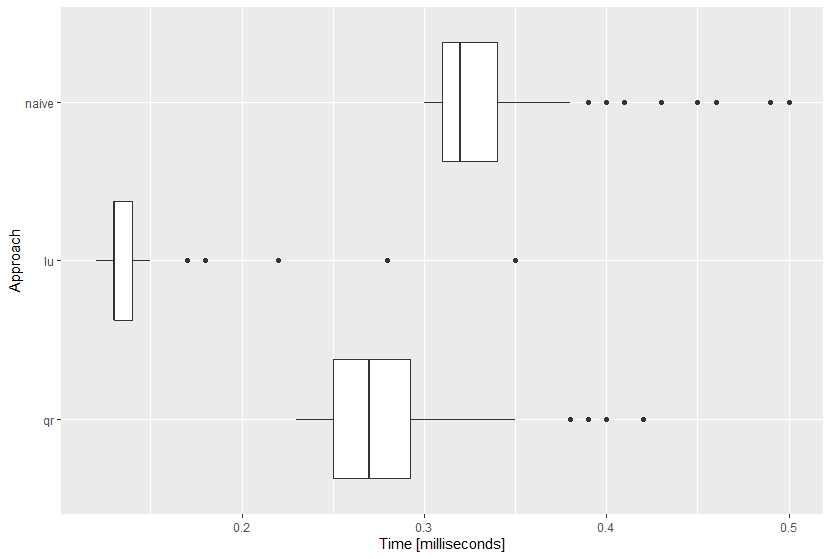
\includegraphics[width = 0.9\textwidth]{figure_man/method_comparison.png} 
\end{center}

% <<echo = F>>=
% set.seed(1)
% X = matrix(rnorm(500*20), 500, 20)
% y = rnorm(500)
% modelBenchmark <- microbenchmark(
%   qr = qr.coef(qr(X), y),
%   lu = solve(crossprod(X),crossprod(X, y)),
%   naive = solve(t(X) %*% X) %*% t(X) %*% y
% )
% @
% 
% 
% <<echo = F, out.width='90%', fig.align='center'>>=
% p = ggplot(modelBenchmark, aes(x = expr, y = round(time/1000000,digits = 2)))+
%   geom_boxplot() +
%   coord_flip() +
%   labs(x = "Approach",y = "Time [milliseconds]")
% p
% @

\end{vbframe}

% \textbf{Problem in der Praxis:}\\
% An sich sehr einfache Berechnung von $\mathbf{R}\boldsymbol{\beta} = \mathbf{Q}^\top\mathbf{y}$.\\
% \medskip
% ABER: $\mathbf{Q}$ nach obigem Algorithmus aus numerischen Gründen oft
% nicht wirklich orthogonal.\\
% \medskip
% {\bf Lösung:} Modifizierte Gram-Schmidt-Ortogonalisierung (MGS), \\
% für Details siehe Monahan bzw.\ Carl D.\ Meyer \emph{Matrix Analysis and Applied Linear Algebra}.
%
% \framebreak
%
% Zwei weitere Methoden für QR-Zerlegung\\
% \medskip
% {\bf Householder Matrizen:}\\
% \medskip
% Für Vektor $\mathbf{u}$ ist Matrix $\mathbf{U} = \mathbf{I} - d\mathbf{uu}^\top$ orthogonal,
% falls $d = 2/ \mathbf{u}^\top\mathbf{u}$.
% Wähle $\mathbf{u} = \mathbf{x} + s\mathbf{e}_1$ mit $s = \mathbf{x}^\top\mathbf{x}$
% $\quad \Rightarrow \quad \mathbf{Ux} = - s\mathbf{e}_1$.\\
% \medskip
% Sukzessive Elimination von Spaltenelementen liefert QR-Zerlegung.\\
% \medskip
% {\bf Givens Matrizen:}\\
% \medskip
% Ähnliches Prinzip zu Householder, aber orthogonale Transformationen, die jeweils
% ein Element eines Spaltenvektors eliminieren, und nur einen zweiten Vektor verändern.\\
% \medskip
% Für Details siehe Monahan bzw.\ Carl D.\ Meyer \emph{Matrix Analysis and Applied Linear Algebra}.


\endlecture
\end{document}







